\documentclass[10pt,a4paper,oneside]{scrartcl}

% \usepackage[ngerman]{babel}   % Deutsches Proposal
\usepackage[USenglish]{babel} % English proposal

\usepackage[utf8]{inputenc}
\usepackage{hyperref,xcolor,microtype,ifthen,csquotes}
\usepackage{graphicx}

\setkomafont{disposition}{}
\setkomafont{descriptionlabel}{\bfseries}

\usepackage[textwidth=450pt]{geometry}

\usepackage[backend=bibtex,style=ieee,hyperref,natbib]{biblatex}

\addbibresource{references.bib}

% Kommentare abschalten
% Disable the hints here
\newboolean{showhints}
\setboolean{showhints}{true}
%\setboolean{showhints}{false}

\newcommand\hint[2]{
\ifthenelse{\boolean{showhints}}{
\begin{center}
\colorbox{black!10}{
\begin{minipage}{.963\textwidth}
#2\hfill\textbf{#1}
\end{minipage}
}\end{center}}{}
}


\newcommand\comment[1]{\textcolor{red}{(#1)}}
% \renewcommand\comment[1]{}

%Title of the proposal
\title{Something Something CouchEdit DSL}
%bachelor or master?
\subtitle{(Bachelor Thesis Proposal)}
%first and then last name
\author{Florian Lappe}

\begin{document}

\maketitle

\section{Introduction and Motivation}
\label{sec:motivation}

% \hint{(this page)}{
% 		An introduction provides readers with the background information for the research proposed (or reported in the paper), with the purpose to provide an understanding of how the research is related to other research \cite{Wilkinson1991}. In an introduction, the writer should \cite{Creswell2008}:
% 		\begin{itemize}
% 		\item Create reader interest in the topic
% 		\item Lay the broad foundation for the problem that leads to the study
% 		\item Place the study within the larger context of the scholarly literature
% 		\item Reach out to a specific audience 
% 		\end{itemize}
% 		}

    Modeling languages have long played an important role in software engineering. Well designed models, can abstract complex systems and provide visual aid in understanding them. Furthermore in form of the Business Process Model Notation (BPMN) they are used to define and automate processes. Today, research in the area of Model Driven Engineering (MDE), a paradigm centered around models, with the intent to generate code bases and whole systems from them, the importance of models is rising even more.

    As these tasks require syntactic correctness of used models, modeling tools become an essential part of an engineers workflow. Especially visual modeling tools provide -in theory- an intuitive and user friendly way to design models. But, current graphical modeling tools, tend to constraint users in unintuitive ways and deliver sub par user experience (UX). This usually arises from a tight coupling between a modeling tools User interface (UI) and the underlying model. As the models syntax is usually unflexible, the UI has to make amends to adhere to this syntax. this often creates problems for the user like, connections can only be drawn between two existing states, or deleting a node will result in all its children being deleted as well.

    To amend these usability woes, L. Nachreiner proposed a novel modeling framework, called CouchEdit \cite{nachreiner_couchedit_2020}. This framework decouples user interface and model syntax by introducing different models for both. Instead of relying directly on the syntax of the model that is being designed, in the CouchEdit architecture, the user interface is using a render model, that only consists of of nodes that are rendered in the Modeling tool, called concrete syntax. On the other hand, the actual models syntax now stands on its own, called abstract syntax. To translate between concrete and abstract syntax, a syntax meta model is utilized. CouchEdit in its core was designed, to be general purpose, meaning it can be rewritten to adhere to any model syntax. But to realize this in the current implementation, the source code has to be rewritten directly, which is error prone, convoluted and requires some understanding of the CouchEdit architectures internal architecture.
    
    To create a more developer friendly and flexible way of adapting CouchEdit to different modeling syntaxes, this design research aims to propose a new 
    domain specific language (DSL), that can be used to configure CouchEdit for 
    any Modeling syntax. Furthermore a conceptual parser is to be developed and implemented, that provides proof of concept how this newly developed DSL interacts with the CouchEdit architecture.

    \comment{questions: who is the audience? Larger context of scholarly litratur?}

\section{Problem Statement}
\label{sec:problem_statement}

\hint{(0,75 pages)}{
		The statement of the problem is the foundation for the construction of any research proposal. In addition to being an integral part of selecting a research topic, it also helps to select research design. It serves as the bases for determining research objectives, formulation of research hypotheses or research questions, and planning the research design \cite{Booth2003}. It allows the researcher to describe the problem systematically, to reflect on its importance, its priority and to point out why the proposed research on the problem should be undertaken. 
		
		A problem might be defined as the issue that exists in the literature, theory, or practice that leads to a need for the study. It is important in a proposal that the problem stands out and that the reader can easily recognize it. 
		\begin{itemize}
		\item A problem statement should be presented within a context, and that context should be provided and briefly explained, including a discussion of the conceptual or theoretical framework in which it is embedded. 
		\item Clearly and succinctly identify and explain the problem within the framework of the theory or line of inquiry that supports the study. 
		\item State the problem in terms intelligible to someone who is generally sophisticated but who is relatively uninformed in the area of your investigation.
		\end{itemize}
		
    Effective problem statements answer the question: Why does this research need to be conducted? If the writer is unable to answer this question clearly and succinctly, the statement of the problem will be perceived as vague and diffuse.}

    \comment{unclear: problem reduziert sich momentan auf: Couchedit framework hat keine schnittstelle um vernünftig neue model syntax zu definieren weshalb DSL benötigt wird. höhere genauigkeit wird benötigt}

\section{Purpose of the study}

% \hint{(0,25 pages)}{The purpose statement should provide a specific and accurate summary of the overall purpose of the study. Briefly define and delimit the specific area of the research. Incorporate the rationale for the study. A commonly used sentence starts with: ''The purpose of this study is \ldots''. The purpose should clarify who is anticipated to benefit from the results of your study and how the results may be used.}

The purpose of this study is to develop a domain specific language, for the CouchEdit Framework. This DSL is supposed to provide a comprehensive and easy to use way for defining new modeling language syntax. Furthermore a prototypical parser is to be implemented, that can comprehend this newly designed DSL and translate it into a set of CouchEdit processors. An explanation about the CouchEdit frameworks processor architecture can be found in the related works section (\ref{CouchEdit}).

This extension of the CouchEdit framework is supposed to improve developer accessibility and framework flexibility, as the implementation of an external DSL and its corresponding parser means, that the system does not have to be recompiled from source code every time a different modeling syntax is to be used. Furthermore in the current implementation, to support new modeling syntax, the user is forced to write processors on source code level, which is convoluted and requires understanding of most of the CouchEdit architecture. By designing a comprehensible DSL syntax, users will have an easier time defining new modeling syntax. 



\section{Review of the literature}

% \hint{(1 page)}{
% 		The literature review provides the background and context for the research problem. It should establish the need for the research and indicate that the writer is knowledgeable about the area. The literature review: 
% 		\begin{itemize}
% 		\item Describes the results of other studies that are closely related to the study being proposed (or reported)
% 		\item Relates a study to the larger, ongoing dialogue in the literature about a topic, filling in gaps and extending prior studies 
% 		\item Provides a framework for establishing the importance of the study, as well as a benchmark for comparing the results of a study with other findings
% 		\item “Frames” the problem earlier identified
% 		\end{itemize}
% 		The literature review should demonstrate to the reader that you have a comprehensive grasp of the field and are aware of important recent substantive and methodological developments. Define the starting point for your study - how will your study refine, revise, or extend what is now known? 
		
% 		In a proposal, the literature review is generally brief and to the point. Select and reference only the more appropriate citations. Make key points clearly and succinctly. Later in your thesis, you will elaborate on this section.
		
		
% 		Initial literature related to the specific topic. This will be a small selection of papers relevant to the work, agreed on with the supervisor. The purpose of this section is to demonstrate problems or limitations of existing solutions.}

\subsection{CouchEdit}
\label{CouchEdit}

As the cornerstone this research builds upon, CouchEdit is of great significance. CouchEdit falls under the category of relaxed conformance editing, meaning, it allows for temporary inconsistencies between concrete syntax (what the user draws) and abstract syntax (what the underlying Model actually looks like). As the concrete syntax does not always have to map to a syntactic correct abstract model, it allows for more freedom in the modeling process, for example, dangling transitions. 

CouchEdit realizes this by building upon the architecture concept of clear separation between concrete and abstract syntax, proposed by Y. Van Tendeloo et al. \cite{van_tendeloo_concrete_2017}. Internally, CouchEdit builds a hypergraph, that maps the given concrete syntax to all possible abstract syntaxes (interpretation of a concrete syntax can be ambiguous and thus multiple abstract syntaxes can be possible). To build this Hypergraph, a set of Processors is employed, which are connected in a reactive publish and subscribe pattern. All Processors -and the user interface- are subscribed to a bus (fig. \ref{fig:processors}). If a change is published to the bus (e.g. the user adds a node to the concrete syntax), all processors that are subscribed to this type of change are notified and calculate new resulting changes, these new changes are then also published to the bus and all processors interested in these new changes are invoked. 

\begin{figure}
	\label{fig:processors}
  \centering
  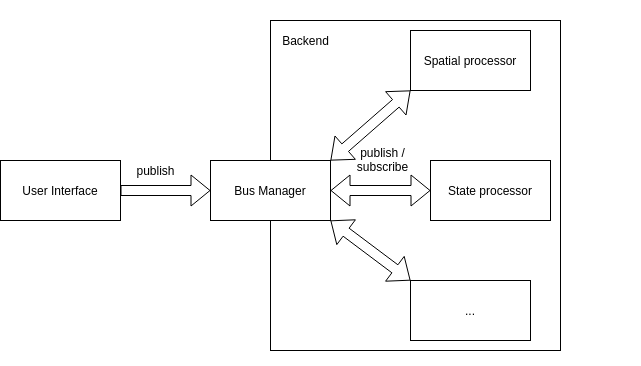
\includegraphics[width=.6\linewidth]{./couchedit-processors}
	\caption{Publish Subscribe architecture of CouchEdit}
\end{figure}

Some of these processors are needed for every type of syntax model, for example the spatial processor, that processes how nodes in the concrete syntax are positioned to each other (above, besides, etc.). Other processors are specific to the given Syntax model, for example the state processor for a state chart syntax, that processes if a given node represents a state (usually true if the given node is a rectangle with rounded edges). The DSL parser that is part of the proposed design research would need to generate syntax specific processors from the DSL. 


\subsection{DiaGen/DiaMeta}
\label{DiaGen/DiaMeta}

The DiaGen project, similar to CouchEdit strives to provide a form of relaxed conformance visual editing. 

\comment{
  \begin{itemize}
    \item hypergraph based modelling editor generator
    \item allows for definition of moddeling syntax via different means (EMF, designer(??), textual)
    \item solid reference as they already implemented a form of modeling syntax generation from DSLs
    \item 
  \end{itemize}
}

\section{Research questions and/or Hypotheses}
\label{sub:questions}

\hint{(0,25 Pages)}{
		Questions are relevant to descriptive, normative or census type research. (What are relevant factors? How many of them are there? Is there a relationship between them?) Hypotheses are relevant to theoretical research, and when you state hypotheses the reader is entitled to have an exposition of the theory that lead to them (and the assumptions underlying the theory). 
		
		In general, you should be prepared to interpret any possible outcome with respect to the questions or hypotheses. Try to visualize in your mind tables or other summary devices, which you expect to come out of the research, short of the actual data.
		
		
		Research questions describe one or several main questions of the thesis, as well as several subquestions agreed upon with the supervisor. Research questions can be split in several types and are typically W-questions (why, what, how, \dots).\footnote{based on \url{http://www.studieren.at/uni-abc/forschungsfrage-welche-fragetypen-gibt-es} (German).}
%
\begin{description}
\item[Explanation:] Why is something the way it is?
\item[Description:] What do different approaches look like?
\item[Prediction:] How will something develop?
\item[Assessment:] How can the described/explained be assessed?
\end{description}

These questions should be written such that they can be answered within the thesis, and they should fully cover the research problem.
}

\begin{itemize}
  \item How does a DSL, describing the whole CouchEdits feature set, look?
  \item What could an implementation of this DSL in the current CouchEdit architecture look like?
\end{itemize}

\section{The Design - Methods and Procedures}
\label{sec:approach}

\hint{(0,5 Pages)}{
		Any research or problem solving requires a systematic approach with methods and procedures. Indicate the steps you will take to answer every question or to test every hypothesis indicated in the previous section, to solve the problem that you are addressing. There are several research methods, e.g. design research \cite{Collins2004,Vaishnavi2004,Oesterle2011}, case study \cite{Runeson2008, Yin2009}, action research \cite{McKay2001}, Survey \cite{Malhotra1998}, and experiment \cite{Basili1986} just to mention a few. Different research methods and procedures require different descriptions. 
		
		For example for a survey, it becomes vital to describe sampling and instrumentation. The sampling, i.e. the population and how the sample has been drawn from that, needs to be described to clarify to what extent the findings of a study can be generalized to people or situations. You should also outline the instruments you propose to use (surveys, scales, interview protocols, observation grids). For a case study or a design research, other aspects become vital. 
		
		\textit{Data collection}
		For all studies, you need to have a systematic approach for data collection. Outline the general plan for what data to collect, and how. This may include survey administration procedures, interview or observation procedures. Also, provide a general outline of the time schedule you expect to follow.
		
		\textit{Data Analysis}
		For all studies, you need to have a systematic approach for data analysis. Specify the procedures you will use to analyze your data. If coding procedures are to be used, describe these in reasonable detail. For evaluations, describe the criteria to be used in reasonable detail.  
		
		
    Describe the initial ideas for the thesis and the first steps to answer the research questions. Ideas can be pointers towards promising ideas in the literature (not necessarily read completely) or some sketch of how ideas from the literature may be developed. It does not need to be a concrete idea, but should indicate what will be done in the first weeks after the proposal is done.}
    

\begin{enumerate}
  \item Analysis of CouchEdit framework
      \begin{itemize}
        \item needed modeling features
        \item architectural requirements
      \end{itemize}
  \item Design of DSL
  \item Implementation
  \item Evaluation 
      \begin{itemize}
        \item does the developed DSL cover the whole feature set?
        \item (performance vermutlich nicht relevant?)
      \end{itemize}
\end{enumerate}


\section{Limitations and Delimitations}
\hint{(0,5 pages)}{
A limitation identifies potential weaknesses of the study. Think about your analysis, the nature of self-report, your instruments, and the sample. Think about threats to external or internal validity that may have been impossible to avoid or minimize and explain these. 

Delimitation addresses how a study will be narrowed in scope. This is where you explain the things that you are not doing and why you have chosen not to do them. For example, the literature you will not review (and why not), the population you are not studying (and why not), the methodological procedures you will not use (and why not). Limit your delimitations to the things that a reader might reasonably expect you to do (given your topic and problem statement) but that you, for clearly explained reasons, have decided not to do.}


\section{Significance of the study}
\hint{(0,25 pages)}{Indicate how your research will refine, revise, or extend existing knowledge in the area under investigation. Note that such refinements, revisions, or extensions may have substantive, theoretical, or methodological significance. Think pragmatically.

Most studies have two potential audiences: practitioners and researchers. Think about implications: What implications may the results of the study have on research? What implications may the results of the study have on practice? }



\section{Planning}
\label{sec:planning}

\subsection{Own Background}
\label{sub:background}

\hint{(0,25 Pages)}{Relevant background on methodologies and tools (e.g., process models, appropriate formal models, formal specifications languages, algorithms) from lectures, seminars and jobs. Also write down the necessary skills that need to be learned during the thesis.}

\subsection{Required Resources}
\label{sub:resources}

\hint{(arbitrary length)}{If applicable, a list of required hardware or other resources.}

\subsection{Work packages}
\label{sub:wp}

\hint{(0,25 Pages)}{General description of the work that needs to be done per month. The time plan should be consistent with the research questions (\ref{sub:questions}) and the necessary background (\ref{sub:background}) and potential wait time for resources (\ref{sub:resources}).}

\begin{description}
\item[M1] \dots
\item[M2] \dots
\item[M3] \dots
\item[M4] \dots
\item[M5] \dots
\item[M6] \dots
\end{description}

\subsection{Contingency plan}
\label{sub:contingency}

\hint{(0,5 Pages)}{Possible risks (e.g., no available resources) that can already be estimated before starting the thesis, as well as possible contingency plans.}

\begin{enumerate}
\item Risk \dots %Risk

      Contingency \dots %Contingency

\item Risk \dots %Risk

      Contingency \dots %Contingency
\end{enumerate}

\nocite{*}
\printbibliography

\end{document}

